\section{Implementazione}
\subsection{VanillaCase}
Nella seguente figura è possibile osservare le connessioni logiche tra tre FMU principali: 
\begin{itemize}
	\item \textbf{FMU of the leading car}: questa FMU implementa il comportamento della leading car. Per funzionare non ha bisogno di alcun input da altre FMU e produce in output la posizione della macchina, la velocità e la sua accelerazione. 
	\item \textbf{FMU of the following algorithm}: questa FMU implementa l'algoritmo di inseguimento. Presi in ingresso i parametri di posizione, velocità e accelerazione della leading car ed i parametri di posizione e velocità della following car produce in output l'accelerazione per la following car.
	\item \textbf{FMU of the following car}: questa FMU implementa il comportamento della following carò Per funzionare prende in ingresso l'accelerazione dalla precedente FMU e produce in output la sua posizione e velocità.
\end{itemize}
\begin{figure}[H]
	\centering
	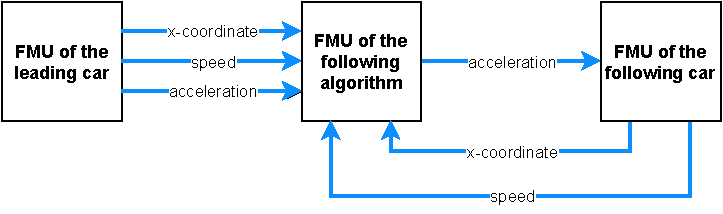
\includegraphics{img/VanillaSchema.pdf}
	\caption{Multi-Model schema del VanillaCase}
\end{figure}

In figura 2 viene rappresentata l'overview del relativo Multi-Model sviluppato con il tool INTO-CPS. 

\begin{figure}[H]
	\centering
	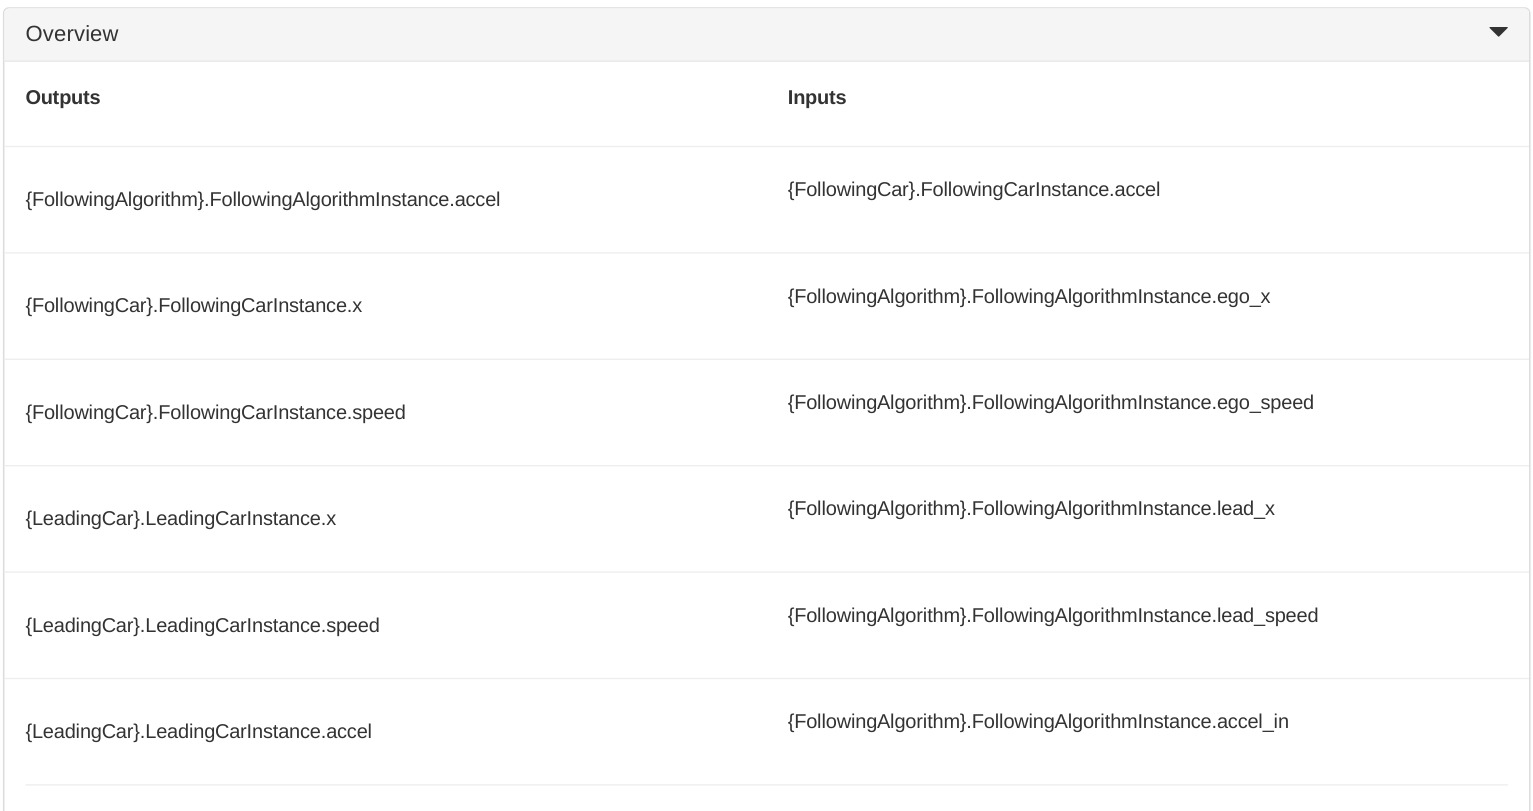
\includegraphics[width=\textwidth]{img/OverviewVanilla.png}
	\caption{Multi-Model Overview del Vanilla Case}
\end{figure}

\subsection{Attacco all'accelerazione}
A differenza dello schema presentato nel VanillaCase, viene ora aggiunto un ulteriore FMU situato fra "FMU of the following algorithm" e "FMU of the following car" già presenti. Il nuovo FMU implementa con strategia \textit{Man-in-the-Middle} un attacco di tipo data alteration sull'accelerazione passata tra il following algorithm e la following car. Fare riferimento alla sezione 3.5 per dettagli sul comportamento dell'attacco.
\begin{figure}[H]
	\centering
	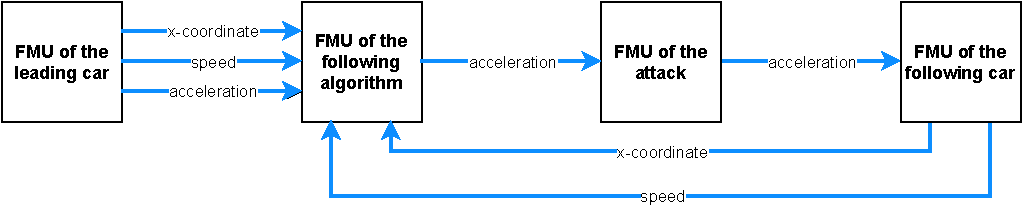
\includegraphics{img/AccelAttackSchema.pdf}
	\caption{Multi-Model schema dell'Attacco alla Accelerazione}
\end{figure}

In figura 4 viene rappresentata l'overview del relativo Multi-Model sviluppato con il tool INTO-CPS. 

\begin{figure}[H]
	\centering
	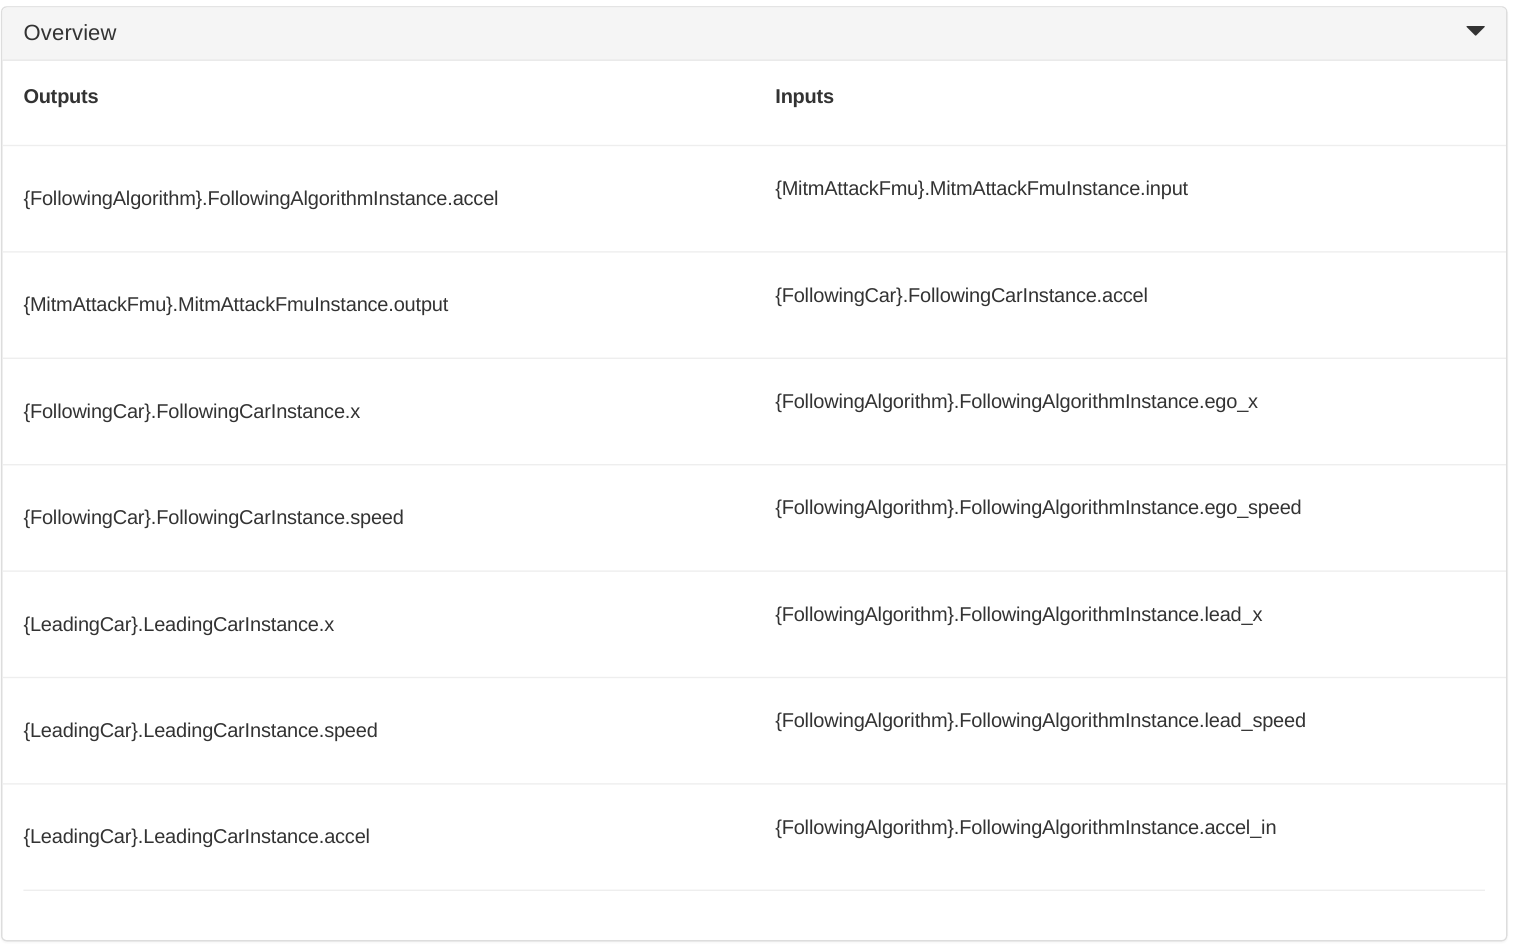
\includegraphics[width=\textwidth]{img/OverviewAccelSingle.png}
	\caption{Multi-Model Overview dell'attacco all'accelerazione (caso attacco semplice)}
\end{figure}
\begin{figure}[H]
	\centering
	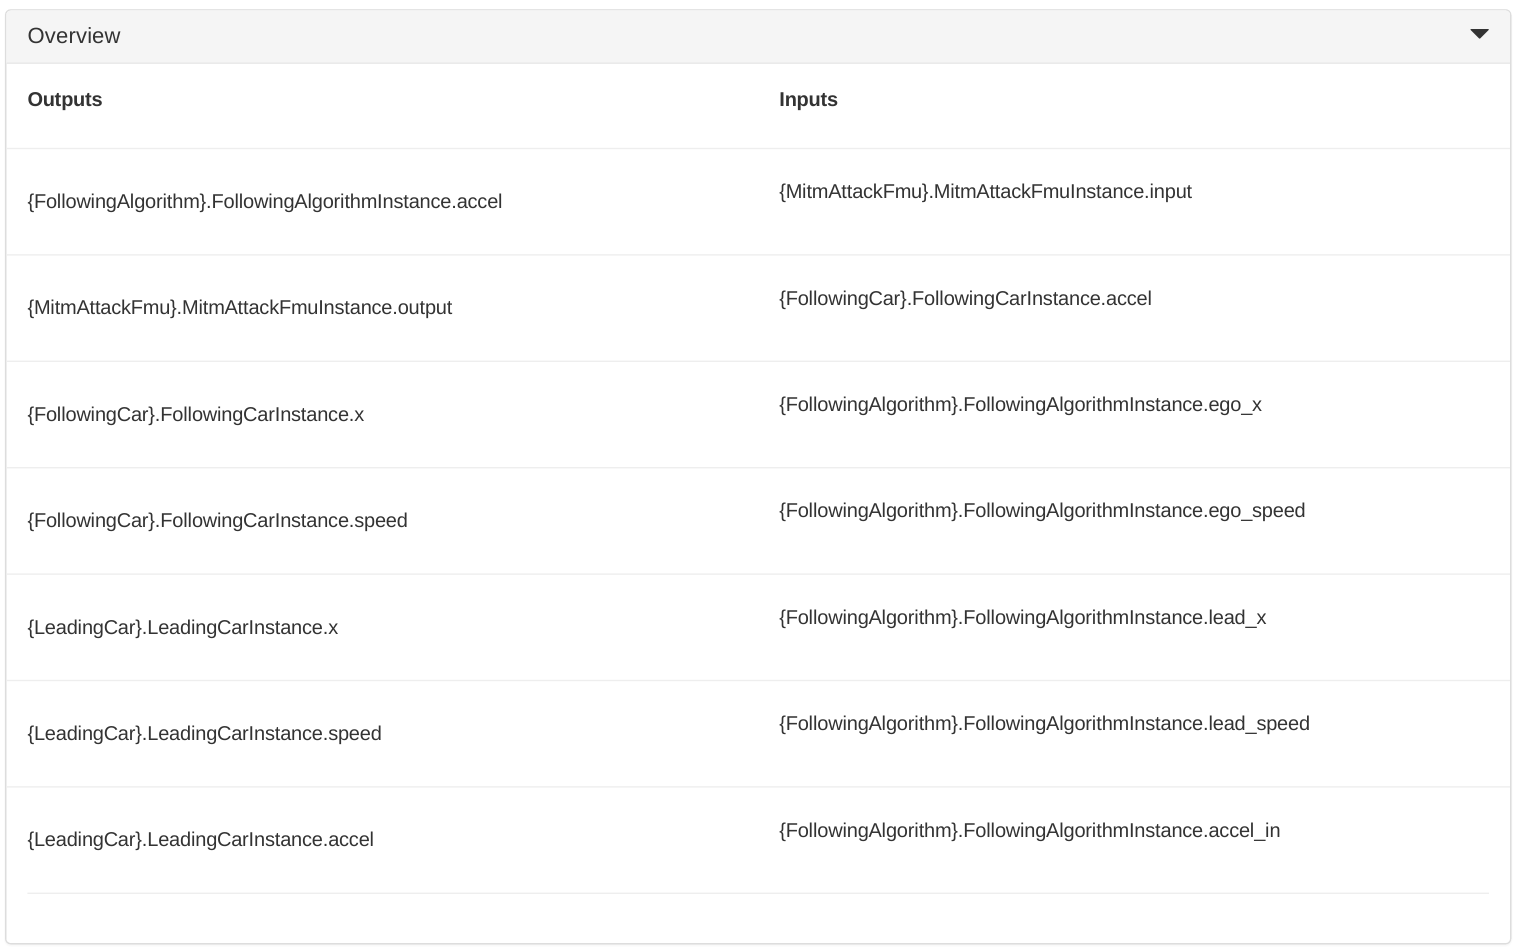
\includegraphics[width=\textwidth]{img/OverviewAccelMulti.png}
	\caption{Multi-Model Overview dell'attacco all'accelerazione (caso attacco multiplo)}
\end{figure}

\subsection{Attacco alla Posizione }
A differenza dello schema presentato nel VanillaCase, viene ora aggiunto un ulteriore FMU situato fra "FMU of the following car" e "FMU of the following algorithm" già presenti. Il nuovo FMU implementa con strategia \textit{Man-in-the-Middle} un attacco di tipo data alteration sulla posizione passata tra la following car e il following algorithm. Fare riferimento alla sezione 3.5 per dettagli sul comportamento dell'attacco.

\begin{figure}[H]
	\centering
	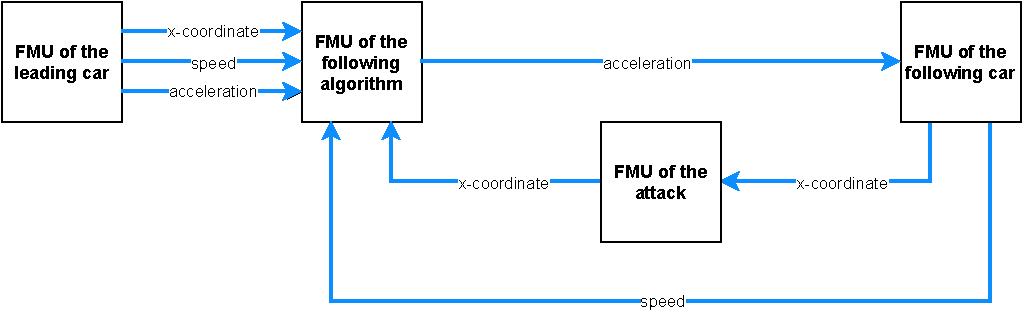
\includegraphics{img/XAttackSchema.pdf}
	\caption{Multi-Model schema dell'Attacco alla Posizione}
\end{figure}

In figura 6 viene rappresentata l'overview del relativo Multi-Model sviluppato con il tool INTO-CPS. 


\begin{figure}[H]
	\centering
	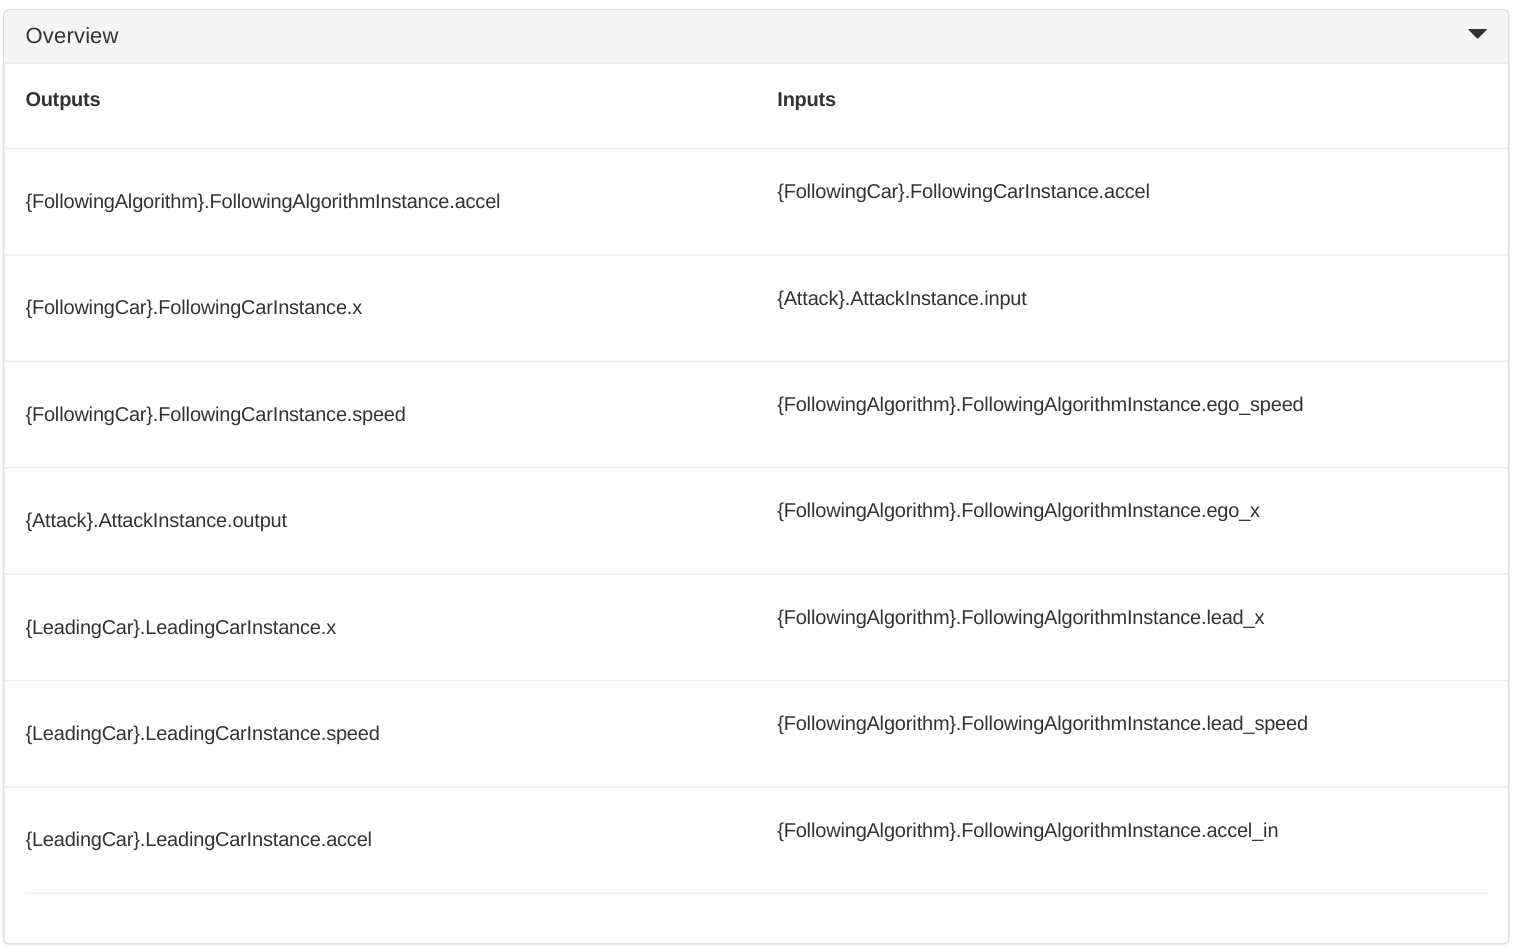
\includegraphics[width=\textwidth]{img/OverviewXSingle.png}
	\caption{Multi-Model Overview dell'attacco alla posizione (caso attacco semplice)}
\end{figure}
\begin{figure}[H]
	\centering
	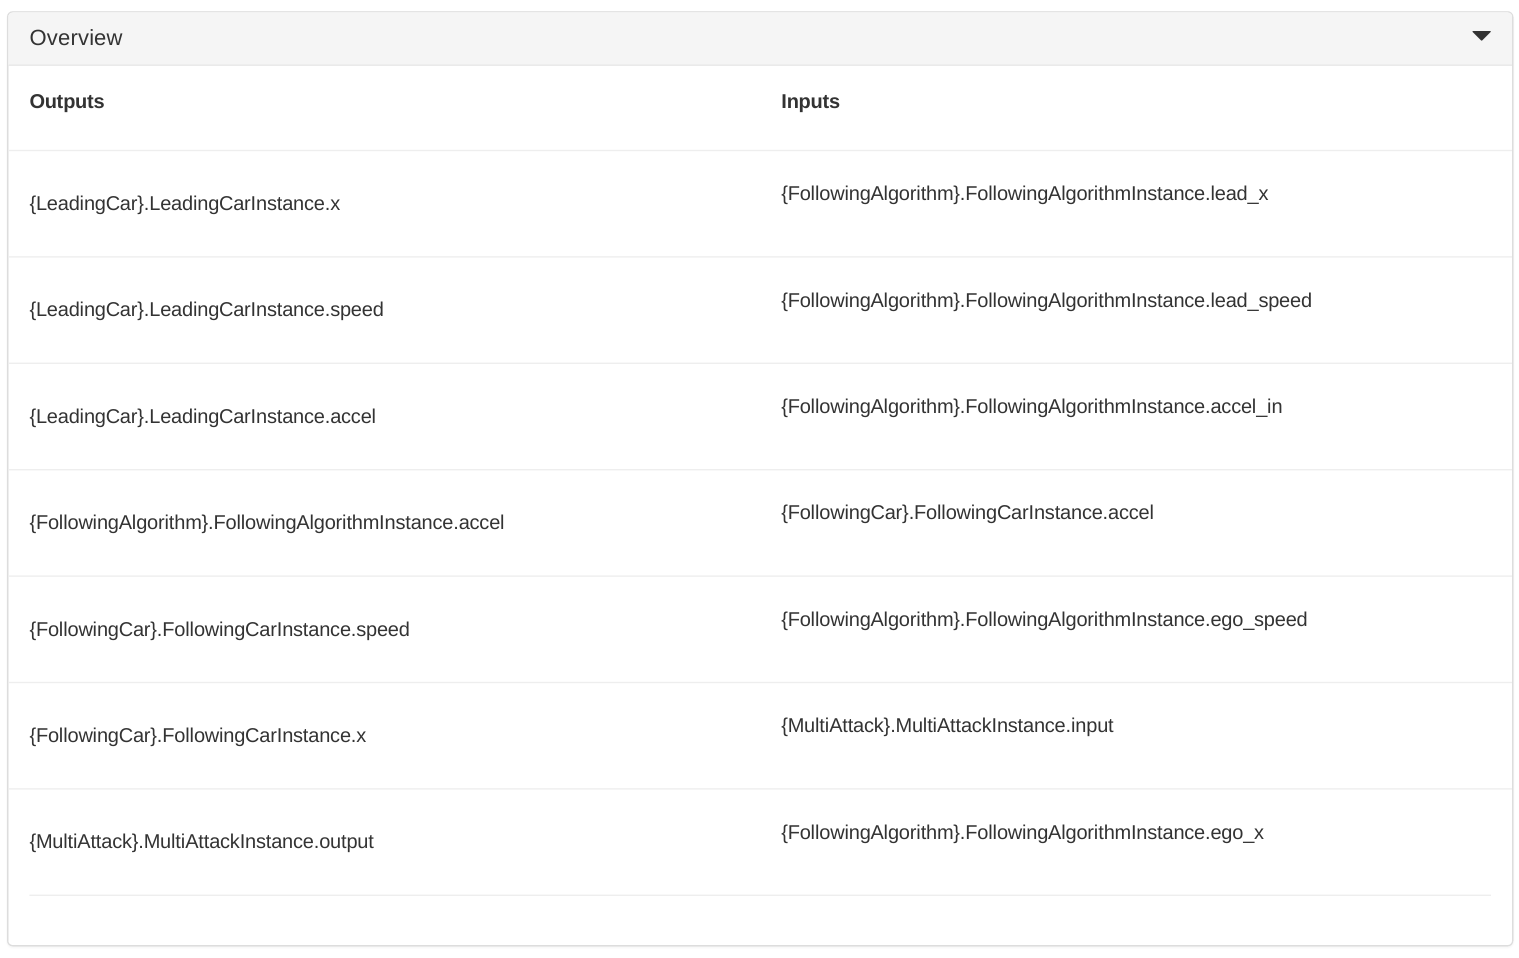
\includegraphics[width=\textwidth]{img/OverviewXMulti.png}
	\caption{Multi-Model Overview dell'attacco alla posizione (caso attacco multiplo)}
\end{figure}

\subsection{Configurazione in Comune}
La configurazione dei seguenti FMU verrà applicata per tutte le simulazioni che verranno effettuate.
\begin{itemize}
	\item \textbf{LeadingCar}:
	\begin{itemize}
		\item Posizione iniziale \textbf{x0}: 50m
		\item Velocità iniziale \textbf{v0}: 0m/s
	\end{itemize}
	
	\item \textbf{FollowingAlgorithm}:
	\begin{itemize}
		\item \textbf{c1}: 0.5
		\item \textbf{eps}: 1
		\item \textbf{omega\_n}: 0.2
	\end{itemize}
	
	
	\item \textbf{FollowingCar}:
	\begin{itemize}
		\item Posizione iniziale \textbf{x0}: 0m
		\item Velocità iniziale \textbf{v0}: 0m/s
	\end{itemize}
\end{itemize}

\subsection{Comportamento degli Attacchi}
L'FMU che verrà utilizzata negli attacchi MITM presenterà due implementazioni diverse:
\begin{itemize}
\item \textbf{Attacco Semplice}: l'attacco consiste nel modificare l'input dell'AttackFMU con il valore del parametro \textbf{attack\_value} dall'istante temporale \textbf{attack\_time} fino al termine della simulazione. Tale valore viene restituito in output dall'AttackFMU. Tale FMU è implementata tramite il file Attack\_fmu.fmu.
\item \textbf{Attacco Multi-step}: l'attacco consiste nel modificare l'input dell'AttackFMU con il valore del parametro \textbf{attack\_value} per un tempo pari a \textbf{attack\_duration}, ripetuto \textbf{attack\_occurrencies} volte e separato nel tempo da \textbf{attack\_distance} secondi. Tale valore viene restituito in output dall'AttackFMU. L'attacco inizierà dall'istante temporale \textbf{attack\_time}. Tale FMU è implementata tramite il file MultiStep\_MultiAttacks\_Fmu.fmu.

\end{itemize}